% TODO titre trop long : viser « Simulations et résultats ».
\section{Évaluation semi-empirique de l'efficacité et de la stabilité}
\label{sec:simulations_numeriques}

Cette section évalue la portée quantitative du mécanisme théorique sur des
instances semi-empiriques. Les profils de trafic et de puissance proviennent
d'équipements Orange d'Île-de-France. Quatre opérateurs virtuels sont
construits autour d'un profil de référence empirique.

L'évaluation répond à trois questions :
\begin{enumerate}
    \item \textbf{Combien d'énergie la coopération économise-t-elle dans les
    instances étudiées ?}
    \item \textbf{À quelle fréquence cette coopération efficace est-elle
    coalitionnellement stable ?}
    \item \textbf{Quels paramètres et mécanismes sont associés au passage
    entre stabilité et instabilité ?}
\end{enumerate}

La section procède en sept étapes. La Section~\ref{subsec:protocole_experimental}
construit les instances et la Section~\ref{subsec:adequation_modele_affine}
calibre leur consommation électrique. La
Section~\ref{subsec:efficacite_operationnelle} mesure les économies, puis la
Section~\ref{subsec:stabilite_grande_coalition} étudie leur partage et sa
stabilité. La Section~\ref{subsec:seuils_capacite_mecanisme} recherche les
mécanismes associés aux différents cas, la
Section~\ref{subsec:sensibilite_mecanismes} fait varier les principales
hypothèses, et la Section~\ref{subsec:limites_evaluation} précise les limites
de l'interprétation.

\subsection{Protocole expérimental}
\label{subsec:protocole_experimental}

Le modèle de la Section~\ref{sec:modele_systeme} demande, pour chaque site,
quatre familles de grandeurs : les demandes horaires \(d_i^h\), les capacités
effectives \(q_i\), les coûts fixes \(F_i\) et les coûts variables unitaires
\(\gamma_i\), le tout satisfaisant \(d_i^h\leqslant q_i\). Le protocole
ci-dessous précise, pour chacune, si elle est observée, estimée à partir des
mesures, ou construite.

\paragraph{Ce qui est observé, calibré, synthétique.}
Les données associent, pour chaque identifiant radio Orange d'Île-de-France,
un trafic descendant horaire, exprimé en Go, et une puissance moyenne,
exprimée en watts. Elles couvrent \(3\,825\) identifiants du lundi 20 au
dimanche 26 mars 2023, soit \(24\times7=168\) créneaux horaires par identifiant et
\(642\,600\) couples trafic--puissance. Dans la suite, chaque identifiant est
traité comme une antenne, et \(\mathcal T\) désigne l'ensemble de ces 168
créneaux. Pour un identifiant et une heure donnés, le trafic et la puissance
sont deux mesures du même équipement ; ils ne sont jamais appariés à partir
de deux antennes différentes.

Une vérification préalable ne met pas en évidence de différence exploitable
entre les deux derniers jours et les cinq premiers : leurs profils moyens par
heure sont presque confondus. De plus, estimer le modèle de puissance sur les
cinq premiers jours plutôt que sur les sept change \(P^{\mathrm{fixe}}\) de
\(1{,}4\,\%\) et \(s\) de \(3{,}5\,\%\) en médiane. Les sept jours sont donc
traités ensemble dans toute la suite.

\begin{table}[htbp]
\centering
\small
\begin{tabular}{p{0.14\textwidth}p{0.33\textwidth}p{0.42\textwidth}}
\hline
Statut & Grandeur & Origine \\
\hline
Observé & trafic et puissance horaires & mesure directe, 168 h, \(3\,825\) antennes \\
Calibré & \(P_i^{\mathrm{fixe}}\), \(s_i\), donc \(F_i\) et \(\gamma_i\) &
régression affine par antenne, Section~\ref{subsec:adequation_modele_affine} \\
Synthétique & association de \(n\) opérateurs sur un site & aucun site
multi-opérateurs n'est observé \\
Synthétique & capacités \(q_i\) & les capacités des antennes admissibles ne
sont pas fournies \\
\hline
\end{tabular}
\caption{Statut de chaque grandeur du modèle.}
\label{tab:statut_grandeurs}
\end{table}

Ces mesures fournissent de vrais profils temporels de trafic et de puissance,
mais n'observent ni plusieurs opérateurs colocalisés, ni la capacité effective $q_i$.
Les instances sont donc semi-empiriques et ne permettent
pas d'estimer la distribution réelle des gains d'un accord entre MNO colocalisés.
Elles permettent toutefois d'étudier, sur des profils ancrés dans des mesures de
terrain, comment le coût optimal \(C_H^*\) défini
en~\eqref{eq:cout_horaire_principal}, le cœur du jeu \((N,v_H)\) de la
Définition~\ref{def:jeu_economies} et la valeur de Shapley dépendent du
trafic, des équipements et des seuils de capacité.

\paragraph{Un plan, puis une instance.}
Un \emph{plan} est un tirage d'antennes, effectué une seule fois. Un
\emph{scénario} fixe ensuite les volumes, les profils temporels, les
équipements, les capacités et le nombre d'opérateurs. Une \emph{instance} est
le site obtenu en appliquant un scénario à un plan. Le même plan produit donc
plusieurs instances, sans nouveau tirage d'antennes.

Pour construire \(n\) opérateurs, une instance utilise \(2n+1\) antennes
réelles distinctes, réparties en trois \emph{rôles}.
L'antenne de référence ne représente pas l'un des \(n\) opérateurs : elle fixe
seulement l'échelle et la composante temporelle commune. Chacun des \(n\)
opérateurs reçoit donc sa propre antenne donneuse, puis sa propre antenne
énergétique.

\begin{table}[htbp]
\centering
\small
\begin{tabular}{p{0.16\textwidth}p{0.48\textwidth}p{0.26\textwidth}}
\hline
Rôle & Ce qu'elle fournit & Nombre par instance \\
\hline
Référence & l'échelle du site, \(\mu_a\), et la composante commune des profils & 1 \\
Donneuse & la composante propre du profil d'un opérateur & \(n\) \\
Énergétique & le couple \((P^{\mathrm{fixe}},s)\), donc \((F,\gamma)\)
d'un opérateur & \(n\) \\
\hline
\end{tabular}
\caption{Les trois rôles. Une antenne n'en joue qu'un dans un même plan.
Pour \(n=4\), une instance nécessite neuf antennes.}
\label{tab:roles_antennes}
\end{table}

Pour toute antenne admissible \(j\), le \emph{profil normalisé}
\begin{equation}
    \phi_j(t)=\frac{d_j(t)}{\bar d_j},
    \qquad
    \bar d_j=\frac{1}{|\mathcal T|}\sum_{t\in\mathcal T}d_j(t),
    \label{eq:profil_normalise}
\end{equation}
vaut en moyenne $1$ sur les 168 heures : il conserve les variations
temporelles de l'antenne, indépendamment de son trafic moyen.

Les facteurs de volume sont construits à partir de la distribution empirique
des trafics moyens \(\bar d_j\) des antennes admissibles. Dans la configuration
de référence illustrée ci-dessous, on prend les quantiles 40, 50, 60 et 75 de
cette distribution, puis on divise les quatre valeurs par leur moyenne. On
obtient ainsi, avant permutation,
les facteurs \(0{,}555\), \(0{,}797\), \(1{,}087\) et \(1{,}562\), dont la
moyenne vaut 1. Une permutation fixée par le plan les attribue aux quatre
opérateurs sans favoriser toujours le même indice.

Chaque opérateur \(i\) reçoit aussi une antenne donneuse \(b_i\). Les trois
niveaux de profils temporels sont construits par
\begin{equation}
    \phi_{i,\ell}(t)
    =(1-\lambda_\ell)\phi_a(t)+\lambda_\ell \phi_{b_i}(t),
    \qquad
    \lambda_\ell\in\{0{,}15,\,0{,}35,\,1\}.
    \label{eq:forme_synthetique}
\end{equation}
Avec \(\lambda_\ell=0{,}15\), les quatre profils sont proches mais non
identiques ; avec \(0{,}35\), ils diffèrent davantage ; avec \(1\), chacun
reprend exactement le profil mesuré de sa donneuse. Les panneaux
(a)--(c) de la Figure~\ref{fig:plan_deroule} montrent ces trois cas sur le
même plan.

La demande de l'opérateur \(i\) est alors
\begin{equation}
    d_i(t)=\mu_a\,\alpha_i\,\phi_{i,\ell}(t),
    \qquad
    \mu_a=\bar d_a,
    \label{eq:demande_synthetique}
\end{equation}
où \(\mu_a\) est le trafic moyen de la référence et \(\alpha_i\) le facteur
de volume relatif de l'opérateur \(i\) : \(\alpha_i=1\) correspond au volume
moyen des quatre opérateurs, et \(\alpha_i=1{,}5\) à un volume supérieur de
50\,\%. Enfin, \(\phi_{i,\ell}\) est son profil normalisé. Comme
\(\sum_i\alpha_i=n\), la somme des demandes moyennes vaut toujours
\(n\mu_a\).

La série \(d_i(t)\) contient bien 168 valeurs. Pour le jour \(j\), la grandeur
notée \(d_i^h\) dans les Sections 3 à 5 est la valeur de cette série au
créneau correspondant à l'heure \(h\) de ce jour. Le calcul journalier utilise
donc 24 valeurs et il est répété pour chacun des sept jours ; la fenêtre
nocturne \(H\) en sélectionne sept par jour.

Les sources du trafic et les sources des paramètres énergétiques sont
tirées séparément. Ce choix est volontaire : dans les données, le trafic
moyen et la puissance fixe sont corrélés à \(0{,}52\), si bien qu'un tirage
commun empêcherait de distinguer l'effet du volume de celui de l'équipement.
Il ne garantit pas que chaque association virtuelle existe réellement. Il
reste néanmoins contrôlé : chaque profil et chaque couple de paramètres
énergétiques proviennent d'antennes admissibles, et les capacités assurent la
faisabilité de toutes les demandes. Cette séparation sert donc à comparer les
mécanismes, pas à reproduire la fréquence réelle de chaque association. Dans
la configuration de la Section~\ref{subsec:efficacite_operationnelle}, les
quatre équipements sont en outre pris dans le même quartile de puissance fixe
afin d'éviter des écarts extrêmes.

\paragraph{Un plan déroulé.}
La Figure~\ref{fig:plan_deroule} et le Tableau~\ref{tab:plan_deroule}
présentent un exemple : la configuration de référence appliquée au premier
plan de la liste gelée. Le tableau conserve les identifiants anonymisés des
antennes utilisées afin que cet exemple puisse être reproduit.

\begin{figure}[!htbp]
    \centering
    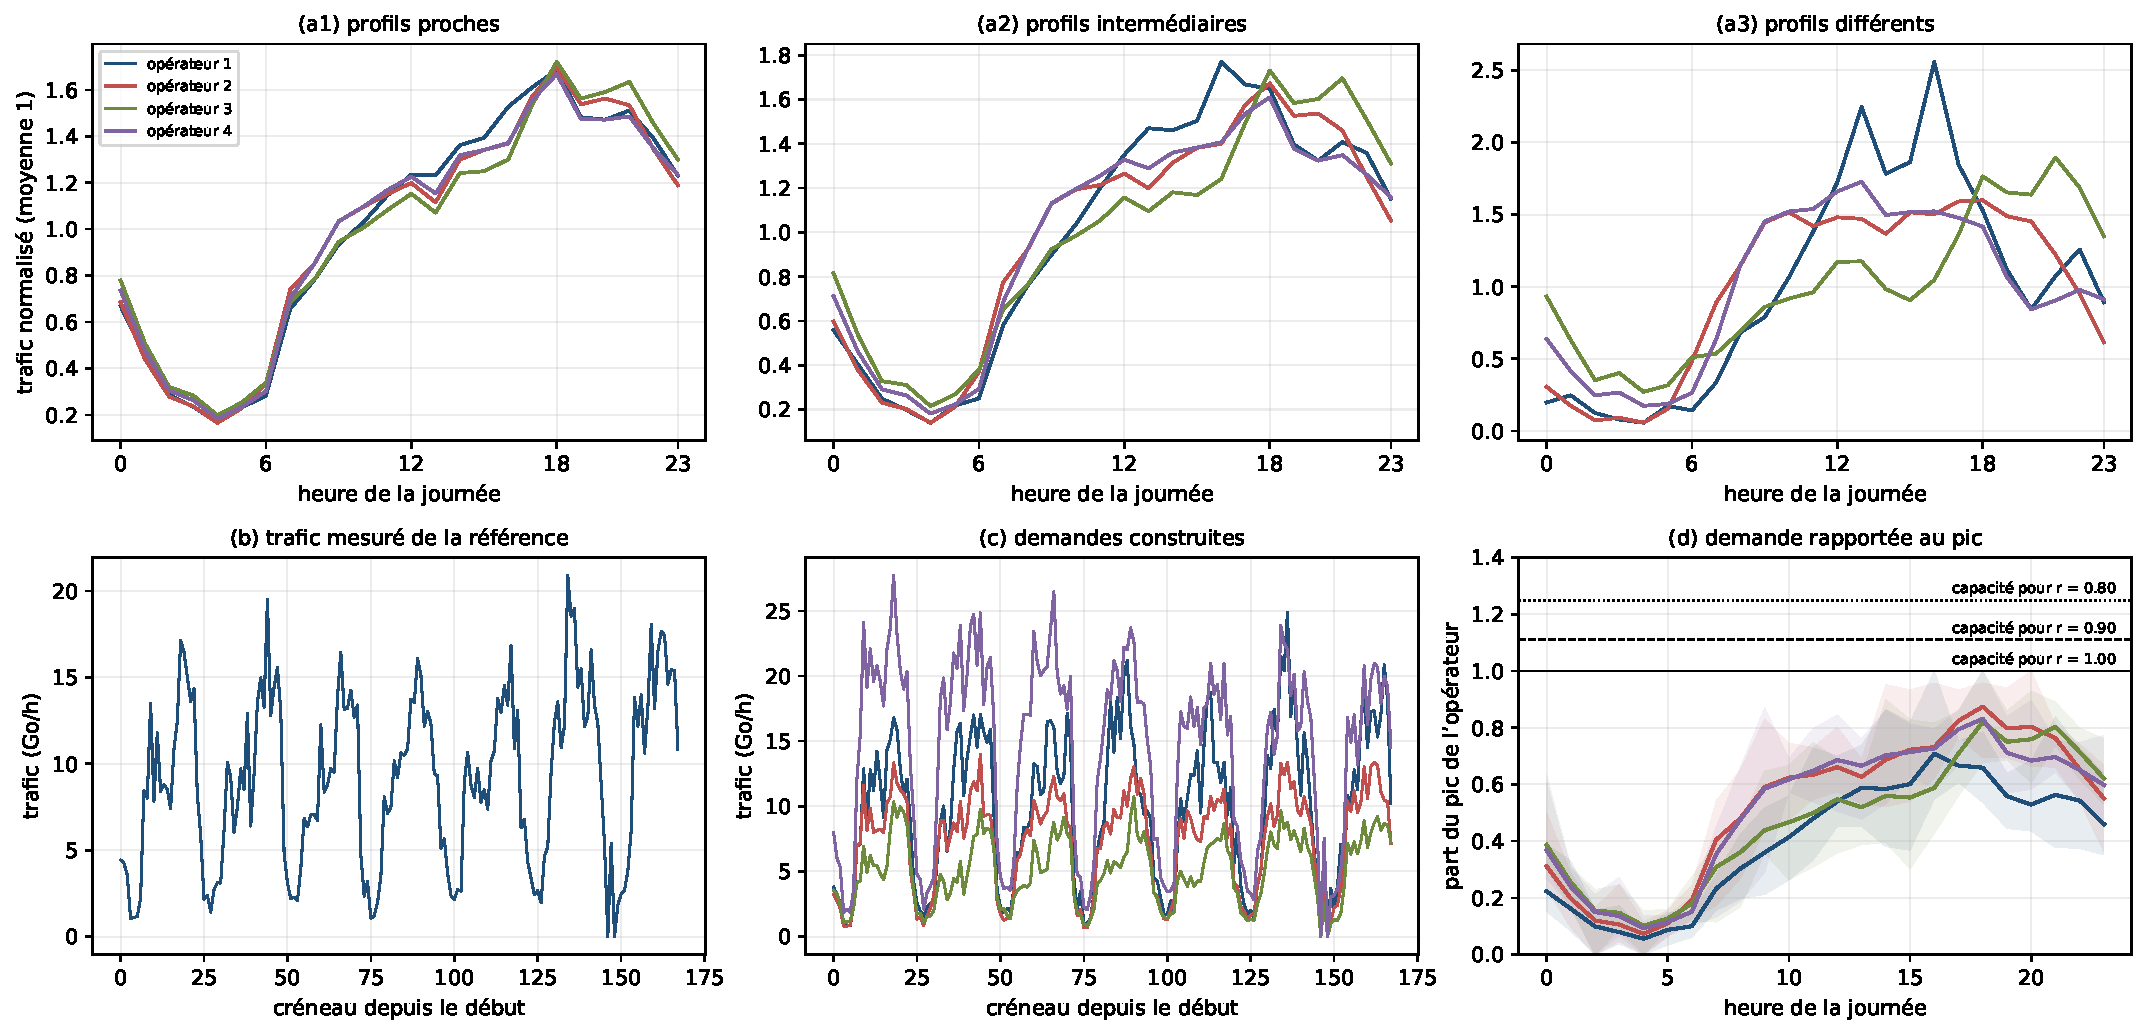
\includegraphics[width=0.98\textwidth]{../figures/protocol/plan_walkthrough.pdf}
    \caption{Construction d'un site virtuel. (a)--(c)~Profils proches,
    intermédiaires et différents, moyennés par heure de la journée ; les
    antennes sources et les volumes ne changent pas entre les trois panneaux.
    (d)~Série réelle de l'antenne de référence sur 168 heures.
    (e)~Les quatre demandes de la configuration intermédiaire construites
    par~\eqref{eq:demande_synthetique}.
    (f)~Demande rapportée au pic de chaque opérateur, plage des sept jours en
    zone colorée, et capacités correspondant aux trois valeurs de \(r\).}
    \label{fig:plan_deroule}
\end{figure}

\begin{table}[!htbp]
\centering
\small
\setlength{\tabcolsep}{3pt}
\begin{tabular}{lrrrr}
\hline
Opérateur & 1 & 2 & 3 & 4 \\
\hline
Antenne donneuse & \texttt{00000493U5} & \texttt{00000244W3} & \texttt{00024518W3} & \texttt{00000204U1} \\
Corrélation avec \(\phi_a\) & \(0{,}908\) & \(0{,}954\) & \(0{,}966\) & \(0{,}894\) \\
Facteur \(\alpha_i\) & \(1{,}087\) & \(0{,}797\) & \(0{,}555\) & \(1{,}562\) \\
Antenne d'énergie & \texttt{00000058W3} & \texttt{00000240U8} & \texttt{00083218W3} & \texttt{00000042U6} \\
\(P_i^{\mathrm{fixe}}\) (W) & \(1\,660{,}9\) & \(1\,758{,}7\) & \(1\,352{,}5\) & \(1\,563{,}7\) \\
Pente (W/Go) & \(41{,}85\) & \(28{,}86\) & \(26{,}62\) & \(24{,}51\) \\
Demande moyenne (Go/h) & \(9{,}96\) & \(7{,}30\) & \(5{,}08\) & \(14{,}31\) \\
Pic \(\max_t d_i(t)\) (Go/h) & \(24{,}90\) & \(13{,}97\) & \(10{,}73\) & \(27{,}70\) \\
\(q_i\) à \(r=0{,}90\) (Go/h) & \(27{,}66\) & \(15{,}52\) & \(11{,}92\) & \(30{,}78\) \\
\hline
\end{tabular}
\caption{Exemple de paramètres d'un site virtuel construit à partir de la
référence
\texttt{00083151W1}, d'échelle \(\mu_a=9{,}16\ \mathrm{Go/h}\). La somme des
demandes moyennes vaut \(36{,}65\ \mathrm{Go/h}\), soit exactement
\(4\mu_a\). Les chaînes alphanumériques sont les identifiants anonymisés des
antennes sources, et non des valeurs numériques.}
\label{tab:plan_deroule}
\end{table}
\FloatBarrier

\paragraph{Variantes contrôlées.}
Cinq réglages font varier les différences entre les opérateurs d'un même
plan : les volumes \(\alpha_i\), les profils temporels, les équipements, le
taux \(r\) et le nombre \(n\). La configuration de référence --- volumes et
profils intermédiaires, équipements issus du même quartile de puissance fixe,
\(r=0{,}90\), \(n=4\) --- est celle du Tableau~\ref{tab:plan_deroule}. On
modifie ensuite un réglage à la fois, en conservant le même plan. Les deux cas
où les trois premières dimensions sont toutes proches ou toutes très
différentes donnent seulement deux contrôles d'interaction.

La dispersion décrit ici les différences entre opérateurs à l'intérieur
d'une instance. Elle n'est pas synonyme de sensibilité : la sensibilité,
étudiée en Section~\ref{subsec:sensibilite_mecanismes}, mesure la variation
du résultat lorsqu'on change un réglage.

\paragraph{Capacités.}
La capacité n'est pas mesurée. On la fixe par un scénario, sous la
contrainte \(d_i^h\leqslant q_i\) de la
Section~\ref{subsec:fenetre_decision} : le pic de la demande construite
occupe une fraction \(r\) de la capacité,
\begin{equation}
    \max_{t\in\mathcal T}d_i(t)=r\,q_i,
    \qquad
    r\in\{0{,}80,\,0{,}90,\,1\}.
    \label{eq:capacite_scenario}
\end{equation}
Ainsi \(r=1\) pose \(q_i\) exactement au pic, et \(r<1\) laisse de la
marge. Changer \(r\) ne reconstruit pas les courbes de trafic : les trois
valeurs partagent les mêmes demandes, et seule la sélection des gardiens
--- quels équipements restent allumés --- peut changer. Par construction,
\(d_i(t)\leqslant r\,q_i\leqslant q_i\), donc aucune heure n'est
individuellement infaisable. Selon les réglages, le nombre minimal de
gardiens observé va de un à quatre ; la
Section~\ref{subsec:seuils_capacite_mecanisme} étudie directement ces quatre
cas.

\paragraph{Fenêtre, réplication et reproductibilité.}
La fenêtre centrale est
\[
    H=\{0\,\mathrm{h},1\,\mathrm{h},\ldots,6\,\mathrm{h}\},
\]
soit \([0\,\mathrm{h},7\,\mathrm{h})\), ses bornes étant un paramètre de
l'analyse de sensibilité. Conformément à~\eqref{eq:cout_horaire_principal},
les gardiens et l'allocation sont recalculés à chaque heure ; l'engagement
persistant de la Section~\ref{subsec:extension_persistante} est traité comme
une contrainte secondaire. Les \(168\) heures sont optimisées séparément, puis
résumées par heure de la journée. Les sept jours sont toujours traités
ensemble, conformément à la vérification donnée au début de cette
sous-section.

La liste gelée contient 400 plans, soit 400 sites virtuels par scénario ; il
ne s'agit pas de 400 sites multi-opérateurs observés. Les antennes de
référence sont tirées sans remise, à raison de 100 par quartile de trafic
moyen. Une graine unique fixe
l'ordre de tous les tirages. À
l'intérieur d'un plan, les sources de trafic et d'énergie sont disjointes ;
une antenne peut réapparaître dans plusieurs plans, jamais deux fois dans le
même. La stabilité des principaux résultats numériques est contrôlée en
comparant les deux moitiés de l'échantillon ; le plan reste toujours l'unité
d'observation.

\paragraph{Diagnostics et contrôles.}
Avant toute interprétation, l'espace d'instances simulé est comparé aux
données d'origine : profils journaliers, autocorrélation de décalage un,
corrélation entre opérateurs d'un même site, distributions des volumes, des
maxima, de \(F_i\) et de \(\gamma_i\), et fréquence des différentes valeurs de
\(k_h\). Ces diagnostics, ainsi que les contrôles croisés de l'implémentation,
sont reportés en Annexe~\ref{app:diagnostics_protocole}. Ces derniers
recalculent chaque optimum par deux méthodes indépendantes : la répartition
gloutonne de la Proposition~\ref{pro:opt} contre le programme
linéaire~\eqref{eq:lp_allocation_fixe}, l'énumération horaire contre le
programme mixte~\eqref{eq:milp_horaire}, la variante persistante
contre~\eqref{eq:milp_gardiens}, le test du cœur contre
Bondareva--Shapley~\eqref{eq:lp_bondareva_shapley}, et l'appartenance du
nucléole au moindre cœur~\eqref{eq:lp_moindre_coeur}. Les contre-exemples
analytiques des Propositions~\ref{prop:contre_exemple_coeur_vide}
et~\ref{prop:shapley_hors_coeur_semi_homogene} sont en outre reproduits
numériquement. Leur rôle est de vérifier que les résultats ne proviennent ni
d'une erreur de construction des instances ni d'une erreur d'implémentation.

\paragraph{Portée.}
Ces instances ne permettent pas d'estimer la distribution réelle des gains
d'un accord entre opérateurs colocalisés, et les capacités y sont
simulées. Elles autorisent en revanche une lecture comparative : à
plan fixé, mesurer comment l'efficacité et la stabilité réagissent lorsqu'on
déplace un seul facteur, tout en restant ancré sur des profils de trafic et
des équipements réellement mesurés.

\subsection{Modèle de puissance}
\label{subsec:adequation_modele_affine}

Le modèle suppose \(P_i(d)=P_i^{\mathrm{fixe}}+s_i d\) pour un équipement
actif. On l'ajuste par moindres carrés, antenne par antenne, sur les
heures à puissance strictement positive des sept jours. Une antenne est
écartée si le trafic ne varie pas, s'il y a trop peu d'heures actives, ou
si \(P^{\mathrm{fixe}}\) ou \(s\) n'est pas strictement positif. Il reste
\(3\,623\) antennes sur \(3\,825\).

L'erreur d'ajustement, rapportée à la puissance moyenne, vaut \(8{,}5\,\%\)
en médiane et reste sous \(15\,\%\) pour \(90\,\%\) des antennes. La part
fixe \(P^{\mathrm{fixe}}/(P^{\mathrm{fixe}}+s\,\bar d)\) vaut \(72\,\%\)
en médiane et dépasse la moitié pour \(93\,\%\) des antennes : éteindre un
équipement économise plus que le report de trafic n'en coûte.

La Figure~\ref{fig:ajustement_puissance} montre trois antennes distinctes,
aux quantiles \(25\,\%\), \(50\,\%\) et \(90\,\%\) de cette erreur :
(a)~bon, (b)~médian, (c)~médiocre. Rouge : \(0\,\mathrm{h}\)--\(6\,\mathrm{h}\) ;
bleu : reste de la journée.

\begin{figure}[htbp]
    \centering
    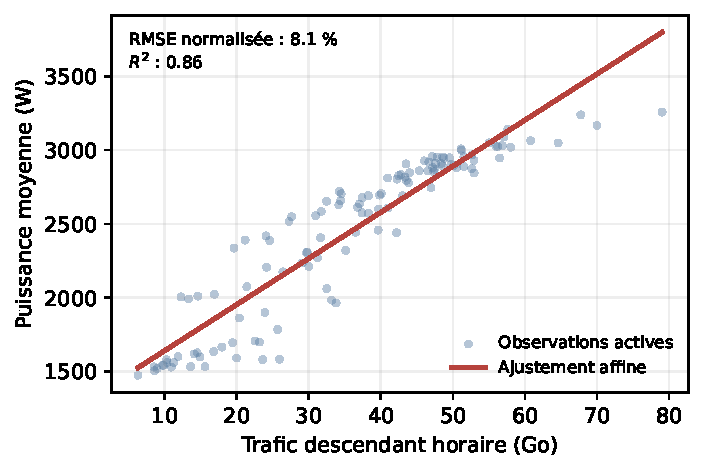
\includegraphics[width=0.95\textwidth]{../figures/power_calibration/representative_power_fit.pdf}
    \caption{Trois antennes distinctes, une par panneau. Droite : ajustement
    affine. Pointillé : \(P^{\mathrm{fixe}}\).}
    \label{fig:ajustement_puissance}
\end{figure}

L'ordonnée à l'origine \(P^{\mathrm{fixe}}\) est la puissance prédite lorsque
le trafic est nul. Elle ne repose pas sur un prolongement lointain de la
droite hors des observations : pour l'antenne médiane, le plus faible trafic
observé ne représente que \(1{,}7\,\%\) de son pic, et \(0{,}8\,\%\) des
heures où la puissance est positive ont exactement un trafic nul. Les données
contiennent donc des points au voisinage immédiat de l'origine.

\paragraph{Deux régimes lorsque l'équipement est actif.}
Le panneau (c), à droite, présente deux groupes de points. Pour un même
niveau de trafic, la puissance mesurée entre 0 h et 6 h est plus faible que
celle mesurée entre 7 h et 23 h ; le rapport entre la seconde et la première
vaut \(1{,}43\) en médiane. Aucune des deux n'est
\(P^{\mathrm{fixe}}\) : ce sont des puissances mesurées pendant que
l'équipement transporte du trafic, tandis que \(P^{\mathrm{fixe}}\) est
l'ordonnée à l'origine de la droite pointillée. Environ \(80\,\%\) des
antennes présentent ce changement de niveau selon l'heure. Le modèle des
Sections 3 à 5 ne distingue qu'un état actif et un état sans trafic ; nous
conservons donc une seule droite par antenne, ajustée sur les 168 heures.

\paragraph{Passage aux coûts.}
On pose \(F_i=\pi P_i^{\mathrm{fixe}}\) et \(\gamma_i=\pi s_i\), avec
\(\pi\) le prix de l'électricité, identique pour tous. Un facteur commun
ne change ni les gardiens ni les économies relatives : on rapporte les
résultats en énergie.

\subsection{Efficacité opérationnelle}
\label{subsec:efficacite_operationnelle}

Cette sous-section étend le calcul du plan déroulé aux 400 plans de
la liste gelée. Pour chacune des trois valeurs de \(r\), cela représente
\(400\) plans observés pendant sept jours, donc \(2\,800\) simulations
journalières. Pour chaque plan et chaque jour, les vingt-quatre coûts
\(C_h^*(N)\) sont obtenus par énumération des quinze ensembles de gardiens et
répartition gloutonne de la Proposition~\ref{pro:opt}.

Nous réutilisons directement le jeu défini en~\eqref{eq:jeu_principal} :
\(v_h(N)\), converti en kWh, est l'énergie économisée par rapport au
fonctionnement autonome, et
\(v_h(N)/\sum_i C_h^*(\{i\})\) est la part économisée. Il n'y a donc pas de
nouveau point de comparaison : le dénominateur reste le coût autonome défini
en Section~\ref{sec:jeu_cooperatif}. Chaque résultat est d'abord
moyenné sur les sept jours d'un plan, puis résumé sur les 400 plans. Dans
les tableaux, les crochets contiennent directement la moitié centrale des
plans, du premier au troisième quartile ; aucun rééchantillonnage ni intervalle
de confiance n'est utilisé.

\paragraph{Profil horaire et choix de \(H\).}
La Figure~\ref{fig:efficacite_operationnelle} suit simultanément la part et
la quantité économisée et le nombre de gardiens effectivement retenus par
l'optimum, \(|G_h^*(N)|\). Les volumes et les profils sont au niveau modéré de
la grille ; les quatre équipements sont tirés dans le même quartile de
\(P^{\mathrm{fixe}}\), avec \(n=4\) et \(r=0{,}90\). Les sept jours sont
traités ensemble selon le protocole de la
Section~\ref{subsec:protocole_experimental}. Le nombre minimal d'équipements
imposé par les seules capacités, \(k_h\), et les conditions suffisantes de
stabilité sont étudiés séparément en
Section~\ref{subsec:seuils_capacite_mecanisme}.

La part économisée médiane vaut \(67{,}6\,\%\) à minuit,
\(76{,}0\,\%\) à 5 h et \(43{,}3\,\%\) à 18 h. L'énergie économisée varie
moins, de \(2{,}22\) à \(3{,}00\,\mathrm{kWh}\) par heure : en journée, le
trafic accroît à la fois le coût du fonctionnement autonome et le nombre de
gardiens retenus par l'optimum.
Le nombre moyen proche de deux vers 18 h signifie seulement que, dans ces
sites virtuels, les capacités simulées de deux équipements suffisent le plus
souvent à servir la demande totale. Il ne s'agit pas d'une mesure du nombre
d'équipements nécessaires sur un site réel.

\begin{figure}[htbp]
    \centering
    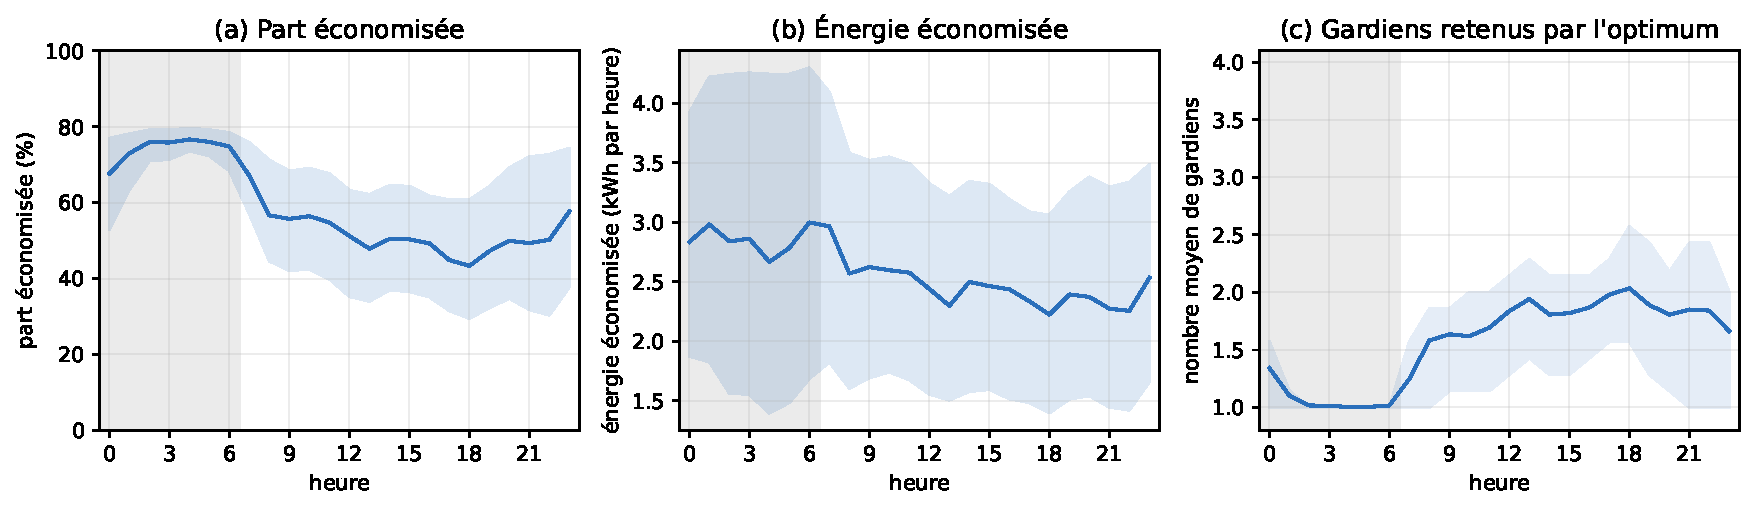
\includegraphics[width=\textwidth]{../figures/operational_efficiency/hourly_profiles.pdf}
    \caption{Profil horaire sur 400 plans, \(r=0{,}90\), les sept jours
    regroupés. (a)--(b)~Part et quantité économisée par rapport au
    fonctionnement autonome. (c)~Nombre de gardiens de l'ensemble choisi par
    l'optimum. Les courbes donnent la médiane des plans et les zones colorées
    leur moitié centrale ; la zone grise est la fenêtre nocturne étudiée.}
    \label{fig:efficacite_operationnelle}
\end{figure}

La fenêtre \(H=\{0,\ldots,6\}\), représentée en gris, a été fixée avant ces
résultats et non choisie en fonction du niveau d'économie observé.

\paragraph{Fenêtre et capacité.}
Le Tableau~\ref{tab:plan_quatre_r} compare les mêmes demandes pour les trois
valeurs de capacité fixées par~\eqref{eq:capacite_scenario}. Accroître \(r\)
de \(0{,}80\) à \(1\) réduit la part économisée de \(1{,}1\) point ; l'énergie
économisée varie de moins de \(0{,}8\,\mathrm{kWh}\) par nuit.

Dans les tableaux de cette sous-section, la notation
\(m\,[q_{25};q_{75}]\) donne la médiane \(m\), puis les premier et troisième
quartiles. Par exemple, \(73{,}7\,[66{,}5;78{,}3]\) signifie que la médiane
des 400 plans vaut \(73{,}7\,\%\) et que leur moitié centrale se trouve
entre \(66{,}5\,\%\) et \(78{,}3\,\%\).

\begin{table}[htbp]
\centering
\small
\setlength{\tabcolsep}{4pt}
\begin{tabular}{ccc}
\hline
\(r\) & Part économisée (\%) & Énergie économisée (kWh/nuit) \\
\hline
\(0{,}80\) & \(74{,}4\ [67{,}1;78{,}4]\) & \(20{,}5\ [11{,}9;29{,}9]\) \\
\(0{,}90\) & \(73{,}7\ [66{,}5;78{,}3]\) & \(20{,}0\ [11{,}9;29{,}6]\) \\
\(1\)      & \(73{,}3\ [65{,}6;78{,}0]\) & \(19{,}7\ [11{,}8;29{,}3]\) \\
\hline
\end{tabular}
\caption{Résultats médians sur les sept nuits. Les crochets contiennent la
moitié centrale des 400 plans. Les demandes sont identiques entre les
lignes.}
\label{tab:plan_quatre_r}
\end{table}

À \(r=0{,}90\), le fonctionnement autonome consomme en médiane
\(30{,}2\,\mathrm{kWh}\) par nuit, contre \(7{,}9\,\mathrm{kWh}\) à
l'optimum. Cet écart est grand parce que le modèle autorise l'extinction
complète : l'optimum ne garde qu'un équipement dans \(93{,}4\,\%\) des heures
nocturnes et évite alors l'essentiel des trois autres coûts fixes. Le terme
fixe représente en médiane \(88{,}6\,\%\) de l'énergie du fonctionnement
autonome sur \(H\). Les quatre puissances fixes sont comparables : la plus
petite représente \(21{,}4\,\%\) de leur somme, contre \(25\,\%\) si elles
étaient identiques. La valeur de \(73{,}7\,\%\) est donc cohérente avec trois
extinctions sur quatre sous les hypothèses du modèle ; elle ne constitue pas
une économie mesurée sur un site réel.

\paragraph{Nombre d'opérateurs.}
Sur les mêmes 400 plans à \(r=0{,}90\), la part économisée passe de
\(66{,}5\,\%\ [59{,}7;70{,}5]\) pour les trois premiers opérateurs à
\(73{,}7\,\%\ [66{,}5;78{,}3]\) pour quatre. La différence appariée médiane
vaut \(6{,}8\ [4{,}6;8{,}1]\) points. Ces valeurs sont proches des
repères homogènes \((n-1)/n\), soit \(66{,}7\,\%\) et \(75\,\%\), car les
puissances fixes sont comparables.

\paragraph{Politiques de référence.}
Trois comparaisons complètent l'optimum horaire. La première allume, à chaque
heure, les équipements par capacité décroissante jusqu'à couvrir la demande,
puis répartit le trafic au moindre coût variable entre eux. La deuxième garde
les équipements de l'optimum, mais répartit le trafic au prorata de leurs
capacités. La troisième impose le même ensemble de gardiens pendant les sept
heures de la nuit, comme dans l'extension persistante de la
Section~\ref{subsec:extension_persistante}.

Pour chaque politique, la Figure~\ref{fig:plan_capacite} contient 400
valeurs : une par plan, après moyenne de ses sept nuits. Le
Tableau~\ref{tab:politiques_operationnelles} résume les comparaisons
appariées plan par plan. Choisir en priorité les équipements de plus grande
capacité ignore leurs coûts et réduit la part économisée de \(3{,}4\) points
en médiane. Imposer le même ensemble de gardiens pendant toute la nuit la
réduit de \(3{,}2\) points.

Les 400 plans utilisent le même réglage, mais pas les mêmes antennes de
référence, donneuses et énergétiques. Pour l'optimum, la moitié centrale des
économies absolues va ainsi de \(11{,}9\) à \(29{,}6\,\mathrm{kWh}\) par nuit.
La part économisée varie moins entre plans, car elle rapporte cette énergie à
la consommation autonome du même plan. Pour la règle par capacité, quatre
plans sur 400 ont même une économie moyenne négative : ignorer les coûts fixes
et variables peut sélectionner des équipements dont la consommation dépasse
la référence autonome. Ces quatre extrêmes sont conservés dans les calculs,
mais pas dans l'échelle des moustaches de la figure.

La politique proportionnelle conserve, à chaque heure, exactement les gardiens trouvés par l'optimum, puis
répartit seulement le trafic entre eux au prorata de leur capacité. Or
\(|G_h^*(N)|=1\) dans \(93{,}4\,\%\) des heures nocturnes : la répartition est
alors imposée et les deux politiques coïncident. Sur les autres heures, la
perte médiane de la répartition proportionnelle vaut \(1{,}14\) point. Son bon
résultat global vient donc surtout du choix préalable des gardiens optimaux,
et non d'une optimalité générale de la règle proportionnelle.

\begin{figure}[htbp]
    \centering
    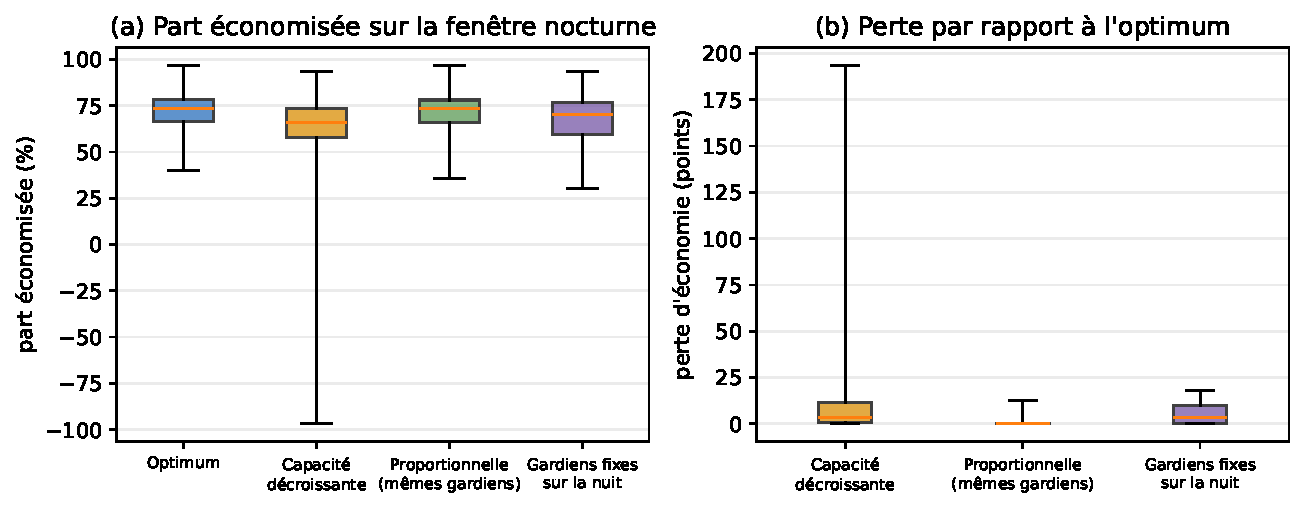
\includegraphics[width=\textwidth]{../figures/operational_efficiency/operational_efficiency.pdf}
    \caption{Résultats des quatre politiques sur 400 plans. Chaque boîte
    résume 400 moyennes, une par plan sur ses sept nuits : le trait orange
    est la médiane, la boîte contient la moitié centrale des plans et les
    moustaches vont des 5\textsuperscript{e} aux 95\textsuperscript{e} centiles.
    (a)~Part économisée par rapport
    au fonctionnement autonome. (b)~Perte appariée par rapport à l'optimum
    horaire.}
    \label{fig:plan_capacite}
\end{figure}

\begin{table}[htbp]
\centering
\setlength{\tabcolsep}{3pt}
\begin{tabular}{lcc}
\hline
Politique & Part économisée (\%) & Perte (points) \\
\hline
Optimum horaire & \(73{,}7\ [66{,}5;78{,}3]\) & --- \\
Capacité décroissante & \(66{,}2\ [57{,}6;73{,}6]\) & \(3{,}4\ [0{,}6;11{,}3]\) \\
Répartition proportionnelle & \(73{,}6\ [65{,}7;78{,}1]\) & \(0{,}002\ [0;0{,}127]\) \\
Gardiens fixes sur la nuit & \(70{,}1\ [59{,}2;76{,}8]\) & \(3{,}2\ [0{,}01;9{,}8]\) \\
\hline
\end{tabular}
\caption{Médianes des 400 plans à \(r=0{,}90\). Les crochets contiennent la
moitié centrale des plans. La perte est calculée plan par plan avant d'en
prendre la médiane ; ce n'est pas la différence entre les deux médianes de la
colonne précédente.}
\label{tab:politiques_operationnelles}
\end{table}

La perte proportionnelle médiane de \(0{,}002\) point est positive mais
presque nulle. Elle ne se déduit pas de \(73{,}7-73{,}6\), car les deux
médianes de la première colonne sont calculées séparément, tandis que la
perte est calculée plan par plan avant d'en prendre la médiane.

L'optimum change d'ensemble \(1{,}14\) fois par nuit en médiane et reste
constant dans \(40{,}6\,\%\) des nuits simulées. La moitié centrale des pertes
dues à la contrainte persistante va de \(0{,}01\) à \(9{,}8\) points : la
reconfiguration horaire importe donc pour une partie des plans.

\paragraph{Année et temps de calcul.}
La moyenne directe des sept nuits observées donne une énergie économisée
médiane de \(20{,}0\,\mathrm{kWh}\) par site et par nuit ; la moitié centrale
des plans va de \(11{,}9\) à \(29{,}6\,\mathrm{kWh}\).
Répétée 365 fois, elle donne \(7{,}3\,\mathrm{MWh}\) par site et par an,
avec une moitié centrale de \(4{,}3\) à \(10{,}8\,\mathrm{MWh}\). La
saisonnalité n'étant pas observée,
il s'agit seulement d'un ordre de grandeur.
Sur la machine de calcul, un site-jour complet --- profil 24 h, trois
politiques et persistance sur \(H\) --- prend environ \(11\,\mathrm{ms}\) pour
\(n=3\) et \(14\,\mathrm{ms}\) pour \(n=4\) ; les \(8\,400\) simulations
journalières sont résolues en environ \(171\,\mathrm{s}\), hors chargement et tracé. Les
résultats intermédiaires sont enregistrés et réutilisés tant que les données,
le protocole et le code de calcul n'ont pas changé.

\subsection{Stabilité et répartition des économies}
\label{subsec:stabilite_grande_coalition}

Nous conservons les 400 plans et les sept heures de \(H\), mais examinons
ici le jeu horaire \(v_h\). Une observation est donc définie par un plan, un
jour, une heure et une valeur de \(r\). Les 400 plans, les sept jours, les
sept heures et les trois valeurs \(r\in\{0{,}80,0{,}90,1\}\) fournissent
\(400\times7\times7\times3=58\,800\) jeux appariés. Cette granularité étudie
une rupture heure par heure. Un cœur vide pour un jeu \(v_h\) n'implique pas
un cœur vide pour le jeu \(v_H\) de la nuit entière : l'agrégation permet aux
gains de différentes heures de compenser leurs contraintes coalitionnelles.
Les deux diagnostics répondent donc à des questions différentes.
Une solution pratique consiste à régler les transferts sur une période plus
longue. Lorsque les 49 heures nocturnes des sept jours sont réunies dans un
seul jeu par plan, aucun des \(400\times3=1\,200\) cœurs n'est vide. À
\(r=0{,}90\), Shapley appartient au cœur pour 378 plans et un autre partage
stable existe pour les 22 autres. L'instabilité horaire ne persiste donc pas
nécessairement lorsque les comptes sont faits en fin de semaine.

\paragraph{Cascade.}
Le test d'appartenance de Shapley au cœur conclut directement pour \(51\,046\)
jeux, soit \(86{,}8\,\%\). Les
\(7\,754\) autres passent au test de non-vacuité du cœur : \(4\,419\) ont un
cœur non vide et \(3\,335\) un cœur vide. Le nucléole n'est calculé que dans
les \(4\,419\) premiers cas, afin d'obtenir le partage stable retenu ; il ne
l'est jamais si Shapley convient déjà. Lorsque le cœur est vide, l'analyse de
la rupture est séparée et le nucléole n'est pas utilisé comme prédiction de
coalition. Sur l'ensemble des 400 plans, le test de Shapley prend \(7{,}3\)
secondes pour les \(58\,800\) jeux et le test du cœur \(17{,}8\) secondes pour
les \(7\,754\) jeux qui l'atteignent, contre \(545\) secondes pour les
\(4\,419\) nucléoles. Ce
dernier étage domine le calcul. Les diagnostics et les partages sont
enregistrés et réutilisés tant que les entrées et le code ne changent pas.

\paragraph{Trois catégories.}
Le Tableau~\ref{tab:stabilite_grande_coalition} donne la répartition des trois
cas. La fréquence de cœur vide passe de \(4{,}6\,\%\) à \(6{,}7\,\%\) lorsque
\(r\) passe de \(0{,}80\) à \(1\), c'est-à-dire lorsque les capacités
\(q_i=\max_t d_i(t)/r\) diminuent. Entre les deux moitiés de 200 plans, l'écart maximal
entre les fréquences des trois catégories n'est plus que de \(1{,}4\) point.

\begin{table}[htbp]
\centering
\setlength{\tabcolsep}{4pt}
\begin{tabular}{ccccc}
\hline
\(r\) & Jeux & \shortstack{Shapley\\stable} &
\shortstack{Autre partage\\stable} &
\shortstack{Grande coalition\\instable} \\
\hline
\(0{,}80\) & \(19\,600\) & \(17\,313\ (88{,}3\,\%)\) & \(1\,378\ (7{,}0\,\%)\) & \(909\ (4{,}6\,\%)\) \\
\(0{,}90\) & \(19\,600\) & \(17\,014\ (86{,}8\,\%)\) & \(1\,477\ (7{,}5\,\%)\) & \(1\,109\ (5{,}7\,\%)\) \\
\(1\) & \(19\,600\) & \(16\,719\ (85{,}3\,\%)\) & \(1\,564\ (8{,}0\,\%)\) & \(1\,317\ (6{,}7\,\%)\) \\
\textbf{Total} & \(58\,800\) & \(51\,046\ (86{,}8\,\%)\) & \(4\,419\ (7{,}5\,\%)\) & \(3\,335\ (5{,}7\,\%)\) \\
\hline
\end{tabular}
\caption{Répartition des jeux horaires de la fenêtre \(H\), sur 400 plans
et avec \(n=4\). « Autre partage stable » signifie que le cœur est non vide
mais que Shapley n'y appartient pas ; le partage retenu est alors le
nucléole.}
\label{tab:stabilite_grande_coalition}
\end{table}

\paragraph{Amplitude de l'instabilité.}
Seuls \(390\) des \(58\,800\) jeux sont convexes, alors que \(86{,}8\,\%\)
admettent Shapley dans le cœur : la convexité est bien une condition
suffisante, non nécessaire. Lorsque le cœur est vide, il faudrait autoriser
chaque coalition à recevoir jusqu'à \(5{,}2\,\%\) de moins que sa contrainte
de stabilité, en médiane, pour rendre un partage possible ; la moitié centrale
de ce manque minimal va de \(2{,}6\) à \(8{,}5\,\%\) de l'économie totale.
Lorsque le cœur est non vide mais exclut Shapley, l'objection
maximale à ce partage vaut \(2{,}77\,\%\) de l'économie en médiane. La
coalition qui objecte compte trois opérateurs dans \(76{,}9\,\%\) des cas et
deux dans les autres. Un test simplifié additionne les exigences des quatre
sous-groupes de trois opérateurs, chacun obtenu en retirant un opérateur. Si
leur somme dépasse ce que la grande coalition peut distribuer, le cœur est
nécessairement vide. Ce test détecte \(65{,}7\,\%\) des cœurs vides, sans faux
positif.

\paragraph{Gains distribués et benchmark de rupture.}
À \(r=0{,}90\), nous additionnons, pour chaque opérateur, les gains qui lui
sont attribués aux sept heures de la nuit. Sur
les \(1\,600\) couples plan--opérateur, le gain moyen est
\(5{,}06\,\mathrm{kWh}\) par nuit, soit \(0{,}76\) euro par opérateur au prix
de \(0{,}15\) euro/kWh, ou \(3{,}04\) euros pour les quatre opérateurs du site.
La médiane est \(5{,}20\,\mathrm{kWh}\) et la moitié
centrale va de \(2{,}90\) à \(7{,}25\,\mathrm{kWh}\). Les numéros
d'opérateur n'étant pas comparables d'un plan à l'autre, nous ne donnons pas
quatre moyennes par identité ; au sein d'un plan, les gains moyens des rangs
le plus faible et le plus élevé valent respectivement \(4{,}49\) et
\(5{,}89\,\mathrm{kWh}\) par nuit.

Lorsque le cœur est vide, le jeu ne prédit pas à lui seul la coalition qui se
formera. Comme benchmark, nous énumérons toutes les partitions propres des
quatre opérateurs, vérifions la stabilité du partage au sein de chaque groupe,
puis retenons la partition stable qui conserve le plus d'économies. Ce
scénario de meilleure partition stable quantifie une perte potentielle ; ce
n'est pas un modèle de formation des coalitions. La perte est mesurée par
rapport au partage de Shapley, hypothétique, de la grande coalition. À
\(r=0{,}90\), les \(1\,109\) cœurs vides sur \(19\,600\) jeux perdent en moyenne
\(0{,}159\,\mathrm{kWh}\) pendant l'heure concernée, avec une médiane de
\(0{,}075\,\mathrm{kWh}\). Cette perte représente en moyenne \(5{,}6\,\%\) de
l'économie de la grande coalition pendant les heures concernées, avec une
médiane de \(4{,}0\,\%\). Rapportée aux \(2\,800\) nuits, ruptures ou non, la
perte collective moyenne est \(0{,}063\,\mathrm{kWh}\) par site et par nuit.
La perte moyenne par opérateur est \(0{,}016\,\mathrm{kWh}\) par nuit ; sa
médiane est nulle et les 5\textsuperscript{e}--95\textsuperscript{e} centiles
vont de \(-0{,}119\) à \(0{,}212\,\mathrm{kWh}\). Une valeur négative signifie
que certains opérateurs bénéficient de la rupture, même si la perte totale est
toujours positive.

Le panneau (b) de la Figure~\ref{fig:stabilite_grande_coalition} ne compare
pas trois politiques énergétiques : dans les trois boîtes, l'économie est
celle de la grande coalition optimale. Les jeux sont seulement classés après
calcul selon leur diagnostic de stabilité ; une économie plus grande ne
garantit donc pas un partage stable.

\begin{figure}[htbp]
    \centering
    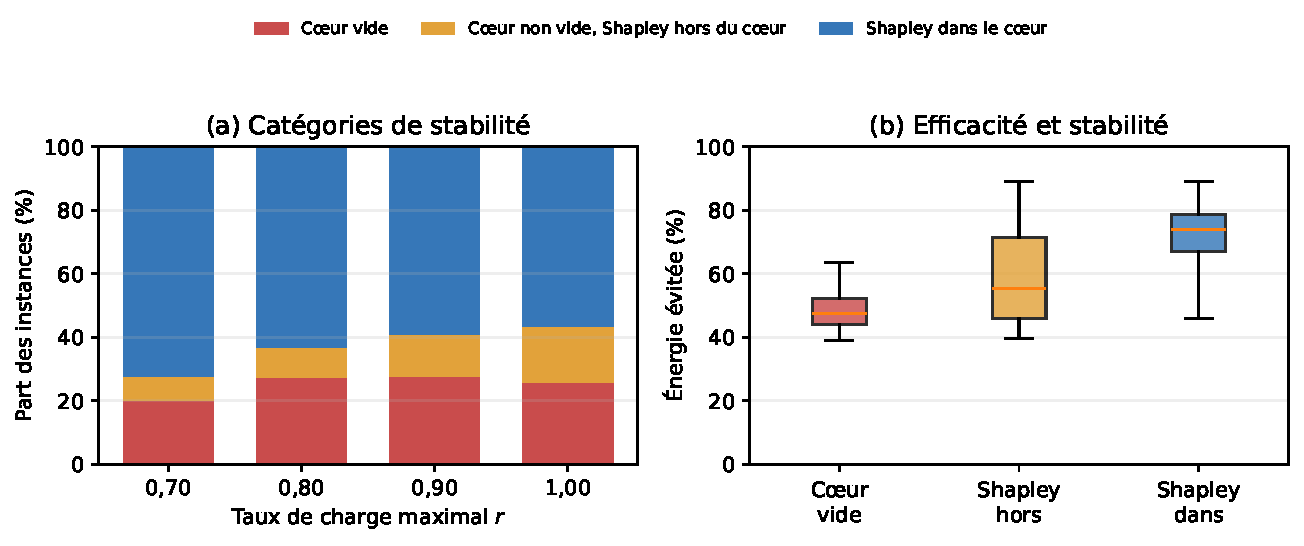
\includegraphics[width=\textwidth]{../figures/coalition_stability/coalition_stability.pdf}
    \caption{Stabilité des \(58\,800\) jeux horaires. (a)~Répartition des trois
    diagnostics selon le taux de charge maximal. (b)~Énergie économisée par
    la grande coalition pendant une heure, c'est-à-dire \(v_h(N)\), classée
    selon le diagnostic. Chaque boîte montre la médiane, la moitié centrale
    et les 5\textsuperscript{e}--95\textsuperscript{e} centiles. Le rouge
    indique un cœur vide, donc une grande coalition instable ; les boîtes ne
    représentent pas des politiques différentes.}
    \label{fig:stabilite_grande_coalition}
\end{figure}

\FloatBarrier

\subsection{Nombre minimal de gardiens et mécanisme}
\label{subsec:seuils_capacite_mecanisme}

La somme sur toute la nuit calculée dans la sous-section précédente peut
masquer les changements du nombre d'équipements nécessaires. Nous revenons
donc au jeu horaire \(v_h\). Pour chacun des 400 plans, nous combinons la
configuration de référence --- volumes et profils intermédiaires, équipements
de puissances fixes proches --- et une configuration où volumes, profils et
équipements sont tous proches. Chacune est évaluée avec les trois valeurs de
\(r\), les sept jours et les 24 heures. Un jeu horaire
est ici entièrement déterminé par un plan et l'une de ces combinaisons. Il y
en a donc
\(400\times2\times3\times7\times24=403\,200\) pour \(n=4\). Le même calcul est
effectué avec les trois premiers opérateurs de chaque plan, soit
\(403\,200\) jeux supplémentaires pour \(n=3\).

Pour interpréter ces jeux, on classe les capacités par ordre décroissant et
on note \(k_h\) le plus petit nombre des équipements les plus capacitaires
dont la capacité cumulée couvre le trafic total à l'heure \(h\). Ainsi,
\(k_h=3\) signifie précisément que les deux plus grandes capacités ne
suffisent pas, mais que les trois plus grandes suffisent. Ce classement
donne un minimum technique, pas le nombre de gardiens effectivement choisi.
L'ensemble \(G_h^*(N)\) peut contenir davantage d'équipements si cela réduit
le coût variable malgré un coût fixe supplémentaire. Ce classement décrit le
régime de charge observé ; il ne constitue pas, à lui seul, une preuve que le
changement de \(k_h\) cause l'instabilité.

\paragraph{Très faible trafic.}
La condition suffisante
\(d^h(N)\leqslant\min_i q_i\) du
Théorème~\ref{thm:capacite_coeur_non_vide} s'applique à
\(138\,200\) jeux à quatre opérateurs (\(34{,}3\,\%\)) et à \(173\,354\) jeux à
trois opérateurs (\(43{,}0\,\%\)). Aucun de ces \(311\,554\) jeux n'a un cœur
vide. Ces pourcentages portent sur les \(403\,200\) observations horaires de
chaque taille de coalition, et non sur 400 plans ou sur des nuits entières.
Dans la configuration de
référence, l'heure la plus favorable est 4 h : la condition est satisfaite
pour \(93{,}4\,\%\) des \(8\,400\) combinaisons plan--jour--\(r\) lorsque \(n=4\),
et pour \(98{,}2\,\%\) lorsque \(n=3\). Les heures 2--6 h sont les plus
favorables dans les deux cas. La condition locale de la
Remarque~\ref{prop:sousadd_stricte_locale}, plus faible, n'est pas comptée ici.

\begin{table}[htbp]
\centering
\begin{tabular}{ccrrr}
\hline
Opérateurs & Gardiens minimaux & Jeux horaires & Cœur vide &
Shapley dans le cœur \\
\hline
3 & 1 & 255\,104 & 2,1\,\% & 94,1\,\% \\
3 & 2 & 128\,992 & 36,0\,\% & 43,5\,\% \\
3 & 3 & 19\,104 & 0,0\,\% & 84,0\,\% \\
\hline
4 & 1 & 219\,194 & 5,5\,\% & 86,1\,\% \\
4 & 2 & 122\,802 & 38,9\,\% & 15,4\,\% \\
4 & 3 & 53\,505 & 59,0\,\% & 20,4\,\% \\
4 & 4 & 7\,699 & 0,0\,\% & 64,1\,\% \\
\hline
\end{tabular}
\caption{Diagnostic des 400 plans selon le nombre minimal de gardiens. Chaque
pourcentage est conditionnel à la ligne correspondante ; la colonne
\emph{Jeux horaires} en donne le dénominateur.}
\label{tab:seuils_capacite}
\end{table}

\paragraph{Nombre minimal de gardiens.}
Le tableau sert à localiser les cœurs vides selon le régime de charge. Par
exemple, \(38{,}9\,\%\) ne concerne que les \(122\,802\) jeux à quatre
opérateurs avec \(k_h=2\), et non l'ensemble des jeux. La fréquence atteint
\(59{,}0\,\%\) pour \(k_h=3\), soit \(31\,572\) cas sur \(53\,505\). Tous
régimes confondus, \(91\,352\) des \(403\,200\) jeux à quatre opérateurs ont
un cœur vide, soit \(22{,}7\,\%\). Ces fréquences sont élevées parce que cette
campagne inclut les 24 heures, trois capacités et deux configurations, et pas
seulement la fenêtre nocturne de référence de la
Section~\ref{subsec:stabilite_grande_coalition}.

Le mécanisme reste celui du contre-exemple théorique : chacun des quatre
sous-groupes de trois opérateurs peut exiger une économie importante, alors
qu'un opérateur appartient à trois de ces sous-groupes. La grande coalition
peut alors manquer d'économies pour satisfaire simultanément les quatre
contraintes. Le test simplifié fondé sur ces quatre sous-groupes
détecte \(76{,}7\,\%\) des cœurs vides pour \(n=4\). Lorsque Shapley est
contestée, la coalition qui présente l'objection maximale est une paire dans
\(37{,}0\,\%\) des cas et un triplet dans \(63{,}0\,\%\). Le cœur vide traduit
une impossibilité de partager les gains de manière stable, non une
infaisabilité technique du service.

Avec trois opérateurs, la condition de très faible trafic est effectivement
plus fréquente et Shapley est stable dans \(77{,}4\,\%\) des jeux, contre
\(55{,}4\,\%\) avec quatre ; le cœur est non vide dans \(87{,}1\,\%\) des
cas, contre \(77{,}3\,\%\). Le gain collectif moyen est en revanche plus
faible : \(1{,}75\,\mathrm{kWh}\) pendant une heure au lieu de
\(2{,}60\,\mathrm{kWh}\). Le cas \(n=3\) confirme donc, sur cet échantillon,
l'intuition d'une stabilité plus fréquente en contrepartie d'un gain total
plus petit. Le lien n'est toutefois pas monotone dans \(k_h\) et le tableau
n'établit pas d'effet causal du nombre minimal de gardiens.

\paragraph{Homogénéité des coûts.}
Nous remplaçons, dans chaque jeu à quatre opérateurs, tous les \(F_i\) par leur
moyenne et tous les \(\gamma_i\) par leur moyenne, puis réintroduisons 25, 50,
75 et 100\,\% des écarts aux moyennes. Le niveau 0\,\% donne donc quatre
opérateurs aux coûts identiques, et 100\,\% restitue les coûts initiaux. Sous
la condition de très faible
trafic, Shapley appartient au cœur dans 100\,\% des jeux à coûts identiques,
comme le garantit le
Corollaire~\ref{cor:shapley_coeur_tres_faible_trafic_homogene}. Cette fréquence
reste supérieure à 99\,\% à 25 et 50\,\% de dispersion, puis tombe à 98,2 et
96,4\,\%. Dès que les coûts diffèrent, le corollaire ne fournit plus de
garantie ; le contre-exemple théorique montre précisément qu'une exception
est alors possible. Sur
toutes les heures, sa fréquence passe de 73,5\,\% à coûts identiques à
60,6\,\% dès le premier quart de dispersion, puis atteint 55,4\,\% avec la
dispersion complète.

\begin{figure}[htbp]
    \centering
    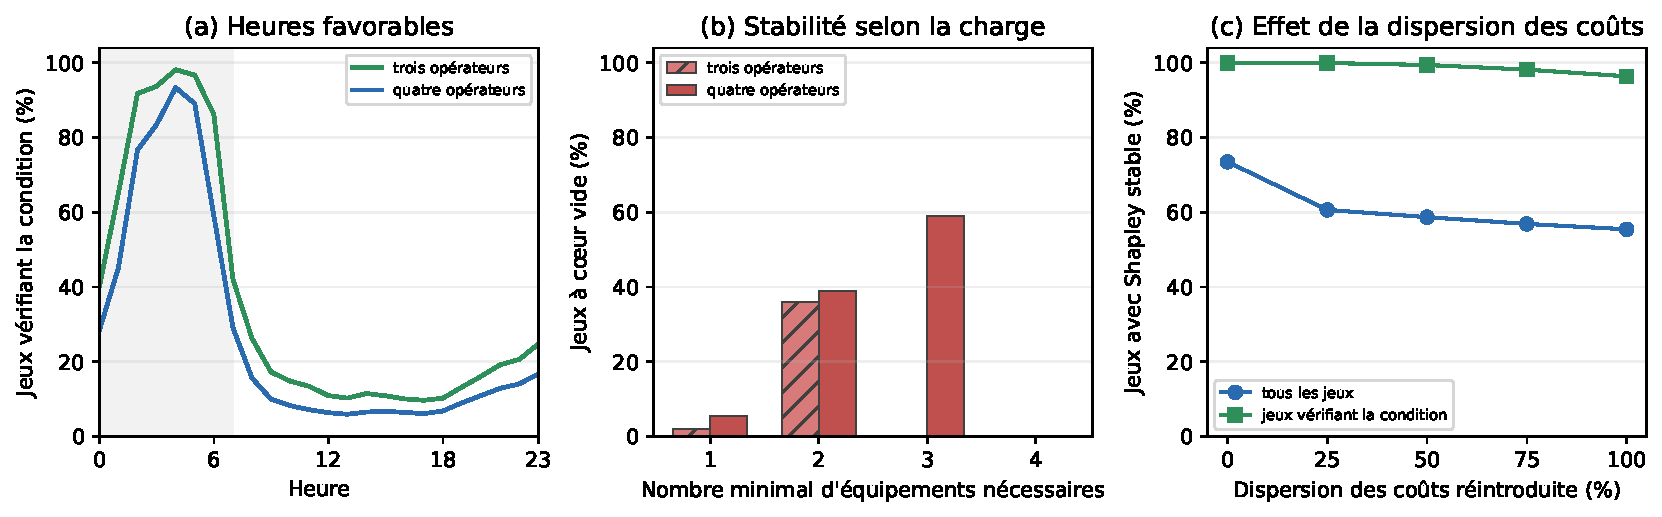
\includegraphics[width=\textwidth]{../figures/coalition_stability/threshold_mechanisms.pdf}
    \caption{Charge et stabilité sur les 400 plans. (a)~Part des \(8\,400\)
    combinaisons plan--jour--\(r\) qui satisfont la condition de très faible
    trafic dans la configuration de référence, selon l'heure et le nombre
    d'opérateurs ; la zone grise indique la fenêtre nocturne.
    (b)~Pour chaque nombre minimal d'équipements nécessaires, part des jeux
    de cette catégorie dont le cœur est vide ; les effectifs sont donnés dans le
    Tableau~\ref{tab:seuils_capacite}.
    (c)~Part des jeux où Shapley appartient au cœur quand les coûts passent
    d'identiques (0\,\%) aux coûts initiaux (100\,\%). La courbe verte porte seulement
    sur les \(138\,200\) jeux de très faible trafic ; seule sa valeur au point
    homogène est garantie par le corollaire.}
    \label{fig:seuils_mecanisme}
\end{figure}

\FloatBarrier

\subsection{Sensibilité}
\label{subsec:sensibilite_mecanismes}

L'analyse revient à la configuration de référence des 400 plans,
avec \(r=0{,}90\), et fait varier un facteur à la fois. Chaque réglage porte
sur \(400\times7=2\,800\) plan--jours ; la position de la fenêtre est comparée sur
les \(400\times6=2\,400\) nuits pour lesquelles
\([22\,\mathrm{h},5\,\mathrm{h})\) est entièrement observée. Avec le trafic
multiplié par 1,2 et les capacités inchangées, 18 plan--jours sur \(2\,800\)
sont hors domaine parce qu'au moins une coalition ne peut plus servir sa
demande. Ils sont signalés comme tels et exclus des statistiques de ce
réglage. Le facteur « veille inactive » modifie la consommation d'un
équipement éteint : elle vaut \(xF_i\), avec \(x\in\{0;0{,}05;0{,}10\}\),
contre zéro dans le modèle de référence. Lorsqu'il est actif, son terme fixe
reste \(F_i\).

Pour chaque plan et chaque réglage, nous moyennons d'abord les jours. Pour un
facteur donné, son \emph{amplitude} sur ce plan est ensuite l'écart entre la
plus grande et la plus petite des trois moyennes. Le
Tableau~\ref{tab:plan_sensibilite} donne la médiane de ces 400 amplitudes. Il
ne donne donc pas le résultat de l'un des trois réglages. Par exemple, \(8{,}10\)
dans la première ligne signifie que, pour chaque plan, on calcule l'écart entre
ses économies sur 22--05, 00--07 et 02--09, puis qu'on prend la médiane des 400
écarts. Une amplitude mesure l'importance du facteur sur la plage testée, mais
ne dit pas à elle seule quel réglage est préférable ; les directions sont
données après le tableau.

\begin{table}[htbp]
\centering
\begin{tabular}{p{3.1cm}p{3.3cm}rrrr}
\hline
Facteur & Valeurs testées & \shortstack{Écart\\d'économie} &
\shortstack{Écart de\\gardiens} & \shortstack{Écart de\\persistance} &
\shortstack{Écart de\\stabilité} \\
\hline
Position de \(H\) & 22--05, 00--07, 02--09 & 8,10 & 0,24 & 7,22 & 0,00 \\
Veille inactive & 0, 5, 10\,\% de \(F_i\) & 6,85 & 0,00 & 0,24 & 0,00 \\
Durée de \(H\), début à minuit & 5, 7, 9 h & 3,15 & 0,07 & 3,23 & 0,00 \\
Niveau de trafic & multiplicateur 0,8, 1, 1,2 & 2,76 & 0,04 & 2,79 & 0,00 \\
Coût fixe \(F_i\) & multiplicateur 0,8, 1, 1,2 & 1,07 & 0,00 & 0,21 & 0,00 \\
Coût variable \(\gamma_i\) & multiplicateur 0,8, 1, 1,2 & 1,05 & 0,00 & 0,20 & 0,00 \\
\hline
\end{tabular}
\caption{Médiane, sur les 400 plans, de l'amplitude entre les trois réglages.
L'économie et la persistance sont en points de pourcentage, les gardiens en
nombre moyen, et la stabilité en points de fréquence des nuits où Shapley
appartient au cœur. Une valeur 0,00 en stabilité signifie qu'au moins la
moitié des plans gardent la même fréquence sur les trois réglages ; elle ne
signifie pas que le facteur n'a aucun effet sur aucun plan.}
\label{tab:plan_sensibilite}
\end{table}

La position de \(H\) a la plus grande amplitude énergétique. La médiane des
moyennes par plan vaut 73,8\,\% sur 00--07, 70,3\,\% sur 02--09 et 67,2\,\%
sur 22--05 : commencer à minuit est donc préférable sur cet échantillon. La
durée compte également, surtout lorsque la fenêtre atteint 9 h : l'économie
médiane vaut 73,6\,\% sur cinq heures, 73,7\,\% sur sept et 70,1\,\% sur neuf.
La définition de \(H\), position et durée, est ainsi le principal choix de la
campagne de sensibilité.

La consommation des équipements inactifs vient juste après : passer de zéro
à 10\,\% de \(F_i\) abaisse l'économie médiane de 73,7 à 67,1\,\%. Le trafic
la fait passer de 75,1\,\% avec le multiplicateur 0,8 à 72,5\,\% avec 1,2,
sur les jeux réalisables. Les multiplicateurs uniformes des coûts fixes et
variables ont chacun une amplitude médiane proche d'un point sur les plages
testées.

Parmi les \(49\,182\) évaluations de jeux nocturnes réalisables, 85 ont un cœur
vide, soit \(0{,}17\,\%\), et Shapley est stable dans \(93{,}3\,\%\) des cas.
Sur les \(2\,800\) jeux du réglage central, le cœur est vide cinq fois et
Shapley est stable dans \(93{,}6\,\%\) des cas. Le trafic fait varier cette
dernière fréquence de 94,9 à 92,3\,\%, et la position de la fenêtre de 91,7 à
93,5\,\%. La médiane des amplitudes par plan reste néanmoins nulle pour tous
les facteurs : au moins la moitié des plans ne changent pas de diagnostic
quand un facteur varie. Contrairement à la Section~\ref{subsec:stabilite_grande_coalition},
ces diagnostics portent sur le jeu nocturne \(v_H\) ; la compensation entre
heures explique que les cœurs vides y soient beaucoup plus rares. Dans ces
plages, l'efficacité opérationnelle est donc nettement plus sensible que la
stabilité de Shapley.

\subsection{Limites}
\label{subsec:limites_evaluation}

Ces fréquences décrivent 400 plans générés à partir du même jeu de données ;
elles ne suffisent pas à estimer la distribution réelle des
gains ni de la stabilité d'un accord entre MNO colocalisés. Les capacités
restent simulées et les mesures couvrent
une semaine, une saison, une région et un opérateur. Le modèle ignore les
coûts de commutation, la qualité de service au-delà de l'écoulement intégral
du trafic, les coûts de transaction et les contraintes réglementaires. La
relation affine unique par antenne ne représente pas les deux niveaux de
puissance active souvent observés selon l'heure ; cette approximation peut
affecter les économies absolues, notamment la nuit, mais conserve la structure
volontairement simple du modèle. Ces ordres de grandeur ne doivent donc pas
être lus comme un bilan industriel.

\FloatBarrier
